%
% This document is based on the Insight Journal Template.
% https://github.com/InsightSoftwareConsortium/InsightJournalTemplate/tree/ModularTemplate
% 4555fc04b105b11f06dc302b76bf09c27e50727d

\documentclass{InsightArticle}

\usepackage[dvips]{graphicx}
\usepackage{listings}
%  hyperref should be the last package to be loaded.
\usepackage[dvips,
bookmarks,
bookmarksopen,
backref,
colorlinks,linkcolor={blue},citecolor={blue},urlcolor={blue},
]{hyperref}

\lstset{ %
language=C++,                % choose the language of the code
basicstyle=\footnotesize,       % the size of the fonts that are used for the code
numbers=left,                   % where to put the line-numbers
numberstyle=\footnotesize,      % the size of the fonts that are used for the line-numbers
stepnumber=1,                   % the step between two line-numbers. If it is 1 each line will be numbered
numbersep=5pt,                  % how far the line-numbers are from the code
backgroundcolor=\color{white},  % choose the background color. You must add \usepackage{color}
showspaces=false,               % show spaces adding particular underscores
showstringspaces=false,         % underline spaces within strings
showtabs=false,                 % show tabs within strings adding particular underscores
frame=single,           % adds a frame around the code
tabsize=2,          % sets default tabsize to 2 spaces
captionpos=b,           % sets the caption-position to bottom
breaklines=true,        % sets automatic line breaking
breakatwhitespace=false,    % sets if automatic breaks should only happen at whitespace
escapeinside={\%*}{*)}          % if you want to add a comment within your code
}


\title{BinShrink: A multi-resolution filter with cache efficient averaging.}

\newcommand{\IJhandlerIDnumber}{3450}

\release{1.01}

% At minimum, give your name and an email address.  You can include a
% snail-mail address if you like.
\author{Bradley C. Lowekamp$^{1}$ and David T. Chen$^{1}$}
\authoraddress{$^{1}$National Library Of Medicine}

\begin{document}

%
% Add hyperlink to the web location and license of the paper.
% The argument of this command is the handler identifier given
% by the Insight Journal to this paper.
%
\IJhandlefooter{\IJhandlerIDnumber}


\ifpdf
\else
   %
   % Commands for including Graphics when using latex
   %
   \DeclareGraphicsExtensions{.eps,.jpg,.gif,.tiff,.bmp,.png}
   \DeclareGraphicsRule{.jpg}{eps}{.jpg.bb}{`convert #1 eps:-}
   \DeclareGraphicsRule{.gif}{eps}{.gif.bb}{`convert #1 eps:-}
   \DeclareGraphicsRule{.tiff}{eps}{.tiff.bb}{`convert #1 eps:-}
   \DeclareGraphicsRule{.bmp}{eps}{.bmp.bb}{`convert #1 eps:-}
   \DeclareGraphicsRule{.png}{eps}{.png.bb}{`convert #1 eps:-}
\fi


\maketitle


\ifhtml
\chapter*{Front Matter\label{front}}
\fi

% The abstract should be a paragraph or two long, and describe the
% scope of the document.
\begin{abstract}
\noindent
We present a new filter for the Insight Toolkit (ITK) for reducing the
resolution of an image by an integer factor while averaging called
\textit{BinShrink}. This filter provides a new level of performance to
ITK for reducing resolution and noise present in an image. The filter
supports streaming, multi-threading and most of ITK's pixel types
including scalars, \textit{Vector}s,
\textit{SymmetricSecondRankTensor}s, and \textit{RGBPixel}s. The
filter has been optimized to efficiently access the input image thereby
greatly increasing performance over conventional methods.
\end{abstract}

\IJhandlenote{\IJhandlerIDnumber}

\tableofcontents

Our new \textit{BinShrink} filter reduces the resolution of an input
image by a integer shrinking factor, while performing averaging of an
input neighborhood. It can be used in streaming processing to reduce
the size of an image that is larger the main memory. The averaging can
effectively reduce uncorrelated noise by reducing the expected
standard deviation by a factor $1/\sqrt{n}$ where $n$ is the number of
samples in the neighborhood, based on the Bienaymé formula.

Electron microscopy  pushes the limits of resolution and detectable
signal, sometimes having less than a 1:4 signal to noise ratio.
The ``binning'' algorithm is commonly used in processing high
resolution electron microscopy images. It is available in packages such
as The Boulder Laboratory for 3-D Electron Microscopy of Cell's
IMOD\cite{IMOD}, and BSoft \cite{bsoft2007}.

In this paper we demonstrate the effective performance improvements which
can be achieved by changing the way an algorithm accesses the data. We
show that by accessing the data is a coherent scan-line order
a 10 times speedup can be realized in some cases.

\section{Implementation}

The algorithm implemented in the \textit{BinShrink} filter can be
described with (Equation \ref{eqn:Algo}) for the 2D case.
\begin{equation}
\label{eqn:Algo}
\mathsf{I}_{out}(x_o,x_1) = \frac{\sum_{i=0}^{f_0}\sum_{j=0}^{f_1}\mathsf{I}_{in}(f_0 x_o+i,f_1 x_1+j)}{f_0 f_1}
\end{equation}

The output image is only defined when all the required input image
pixels are defined. The vector variable $\mathbf{\overline{f}}$ is a user specified
shrink factor.

The method operates only on local input and output regions making the
filter appropriate for streaming. Also the only operations required are
pixel wise addition and division by a scalar, so the filter can readily
work with a wide variety of pixel types.

\subsection{Geometry}

The geometry of an image includes its pixel spacing, origin, and
image orientation. For the \textit{BinShrink} filter the orientation is
unchanged from the input image to the output image, but the output
image's spacing is scaled from the input spacing by the shrink factor.
Also, there is some complication when defining the origin. When the input image size is
not evenly divisible by the shrinking factor, a choice of how to
``round'' the pixel locations needs to be made. We have chosen to maintain the physical
location for the image signal and truncate the odd pixels at the
boundaries. As an ITK image can have non-zero starting indexes, we define
that the output origin pixel must lay on the same lower boundary as the
input, and therefore the origin must be adjusted accordingly (See figure \ref{fig:PixelGrid}).

\begin{figure}
  \centering
  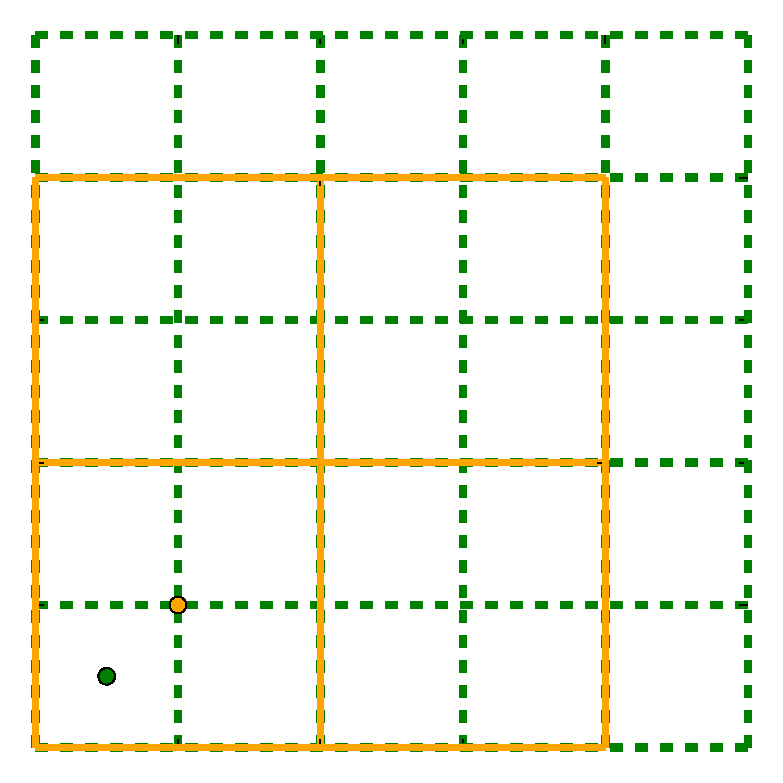
\includegraphics[width=0.4\linewidth]{images/pixelgrid}
  \itkcaption{The change in image geometry from a 5x5 image
    binned by a factor of 2x2. The green dotted lines are the input
    image. The yellow grid is the result of the filter. The points
    represent the respective origins.}
  \label{fig:PixelGrid}
\end{figure}

While this approach maintains the physical location of the image
signal, it does not always maintain either the full extent or the
center of the image. Therefore for algorithms such an image pyramids or certain
neuro-imaging analysis, this method may not be appropriate, or
assurances must be made that the input size is divisible by the shrink factor.

\subsection{Initial Implementation}

We have included the initial, naive implementation of the filter in the
submission for performance comparison purposes and have named it
\textit{BinShrink2}. The above description of geometry applies only to the
\textit{BinShrink} filter. The original \textit{BinShrink2} was
derived from ITK's \textit{Shrink} filter, which has different
geometry characteristics than described above. The original \textit{BinShrink2}
follows the same geometry as the \textit{Shrink} filter.

This original implementation used ITK's conventional
\textit{NeighborhoodIterator} to average the input for each output
pixel (See Listing \ref{lst:01}).

\begin{lstlisting}[label=lst:01, caption={A selected section of code
      from \textit{BinShrink2} filter using the neighborhood iterator.}]
while ( !outIt.IsAtEnd() )
  {
  outputIndex = outIt.GetIndex();

  inputIndex = outputIndex * factorSize + offsetIndex;

  inputIt.SetLocation( inputIndex );

  AccumulatePixelType sum = NumericTraits<AccumulatePixelType>::Zero;
  typename ConstNeighborhoodIteratorType::ConstIterator ci = inputIt.Begin();

  for (ci.GoToBegin(); !ci.IsAtEnd(); ++ci)
    {
    sum += AccumulatePixelType( ci.Get() );
    }
  sum = sum / double( inputIt.GetActiveIndexListSize() );

  outIt.Set( sum );
  ++outIt;
  }
\end{lstlisting}


\subsection{Optimization}

The implementation we suggest for inclusion in ITK is the
\textit{BinShrink}, which follows the geometry described
above (Section 1.1) and is not derived from the \textit{ShrinkFilter}. The initial
implementation accesses the memory in an incoherent fashion based on
the input neighborhood. However, it is faster to access memory in a
linear and coherent fashion. Therefore we designed \textit{BinShrink}
to access the input image on a per scan-line basis and to operate the
averaging on whole scan-lines, not individual pixels. By utilizing ITK's
\textit{ScanlineIterators}, we improved the algorithm to work on a
scan-line for the innermost loops (See Listing \ref{lst:01}).

\begin{lstlisting}[label=lst:02, caption={A selection of code from the
  \textit{BinShrink} filter demonstrating scan-line averaging.}]
while ( !outputIterator.IsAtEnd() )
  {
  const OutputIndexType outputIndex = outputIterator.GetIndex();

  typename std::vector<OutputOffsetType>::const_iterator offset = offsets.begin();
  const InputIndexType startInputIndex = outputIndex * factorSize;

  while ( ++offset != offsets.end() )
    {
    inputIterator.SetIndex( startInputIndex+*offset );

    for( size_t i = 0; i < ln; ++i )
      {
      for( size_t j = 0; j < factorSize[0]; ++j)
        {
        accBuffer[i] += inputIterator.Get();
        ++inputIterator;
        }
      }
    }

    for ( size_t j = 0; j <ln;++j)
    {
      accBuffer[j] = accBuffer[j] * inumSamples;
      outputIterator.Set( static_cast<OutputPixelType>(accBuffer[j]) );
      ++outputIterator;
    }

    outputIterator.NextLine();
  }
\end{lstlisting}

\section{Results}

To test our BinShrink filter we have used a synthetic function
created by Marschner and Lobb\cite{MarschnerL94}, along with additive
noise to create test images. This function is often used to
evaluate volume rendering reconstruction filters. We have rendered it
into a 128 pixel cubic volume such that the majority of the frequencies in
the function are sampled just above 4 times the Nyquist frequency. Such an image
makes for a challenging theoretical data set when the shrinking factor is also
4.

The code used to generate these images was written in Python with
SimpleITK. The original Marshner-Lobb volume was normalized with the
\textit{Normalize} filter so that the volume had a mean
of 0 and a standard deviation of 1. Then Gaussian distributed random
noise was added with a 0 mean and a sigma to achieve the targeted
signal to noise ratio. After the shrinking operation was performed,
the volume was again normalized for contrast. Then the center slice
was extracted and tiled. Finally it was colorized by the
\textit{ScalarToRGBColormap} filter\cite{Tustison2009}.

We examined the results of the \textit{BinShrink} filter by varying the
signal to noise ratio in our Marshnel-Lobb test image and then shrinking those noisy
images by factors of 2 and 4 (See figure
\ref{fig:BinShrinkComparison}). For comparison we also used the
\textit{SmoothingRecusiveGaissian} filter in conjunction with the
\textit{Shrink} filter on the same test noisy images.  We set \textit{sigma} of the
smoothing Gaussian kernel at 0.7 times the shrink factor.

\begin{figure}
  \centering
  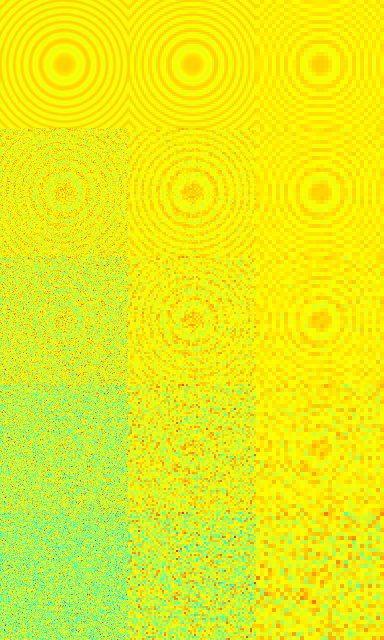
\includegraphics[width=0.4\linewidth]{images/binshrink_hot.png}
  \caption{Outputs of the \textit{BinShrink} filter on a
    Marchner-Lobb function with additive Gaussian noise. The (Left)
    column is the original image, the (Center) column is binned
    by 2, and the (Right) column is binned by 4. The signal to
    noise ratio varies by row with the values 100:1, 2:1, 1:1, 1:2,
    and 1:4, respectively.}
  \label{fig:BinShrinkComparison}
\end{figure}

\begin{figure}
  \centering
  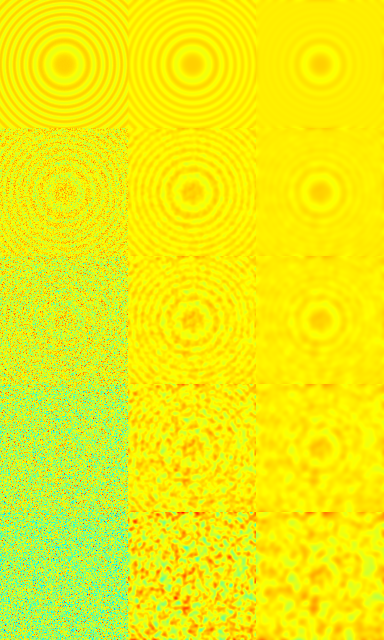
\includegraphics[width=0.4\linewidth]{images/gaussianshrink_hot.png}
  \caption{Outputs of the \textit{SmoothingRecusiveGaussian} and
    \textit{Shrink} filters on a Marchner-Lobb function with additive
    Gaussian noise. The (Left) column is the original image, the
    (Center) column is smooth with a sigma of 1.4 and shrunk by 2, and
    the (Right) column is smoothed by 2.8 and shrunk 4. The signal to
    noise ratio varies by row with the values 100:1, 2:1, 1:1, 1:2,
    and 1:4, respectively.}
  \label{fig:GaussianShrinkComparison}
\end{figure}


Comparing the results of Gaussian filtering (Fig. \ref{fig:GaussianShrinkComparison})
  with \textit{BinShrink}'s box filtering (Fig.  \ref{fig:BinShrinkComparison})
reveals the aliasing that the latter can produce.
This artifact is most apparent in the images with signal to noise ratios of 100:1, the
images in the upper right-hand corner of the two figures.  The Gaussian filter image is much smoother without the banding artifact.


\subsection{Performance}

To analyze the performance of our two bin shrinking methods (both the optimized and naive
  versions) we compare them
against similar processes which can be performed in ITK with other pairs of filters.

Running a \textit{Mean} filter followed by a \textit{Shrink} filter is a
close approximation to \textit{BinShrink}. The
\textit{Mean} filter computes an average for each input pixel's
neighborhood in a brute force fashion. This approach wastes computation on input
pixels that are not used by the \textit{Shrink} filter.

Using a Gaussian kernel to reduce aliasing is another alternative to the box
kernel implicitly used with the \textit{BinShrink} filter. Gaussian filtering can be
performed in constant time and independent of the size of the Gaussian with
the \textit{SmoothingRecusiveGaussian} filter.

We generated a 384 pixel cubic image of Gaussian distributed noise for
performance evaluation. We set the number of threads used to be
16. Utilizing SimpleITK and Python's
\textit{timeit} module, we report the median of 3 runs for each
algorithm across varying shrink factors (See Figure
\ref{fig:ShrinkPerformance} and Table \ref{tab:ShrinkPerformance}).  The image size, the number of threads,
and the shrink factors were carefully chosen such that the output
image was always evenly divided for multi-threading. As expected the
\textit{Mean} approach suffers from exponential cost as a function of
shrink size, while the
\textit{SmoothingRecursiveGaussian} method remains constant. The
\textit{BinShrink2} implementation only touches each input pixel once,
but it also suffers from exponential growth likely due to its memory
access pattern being inefficient and not cache coherent. On the other
hand the \textit{BinShrink} implementation execution time decreases as
the shrink factor increases.

\begin{figure}
  \centering
  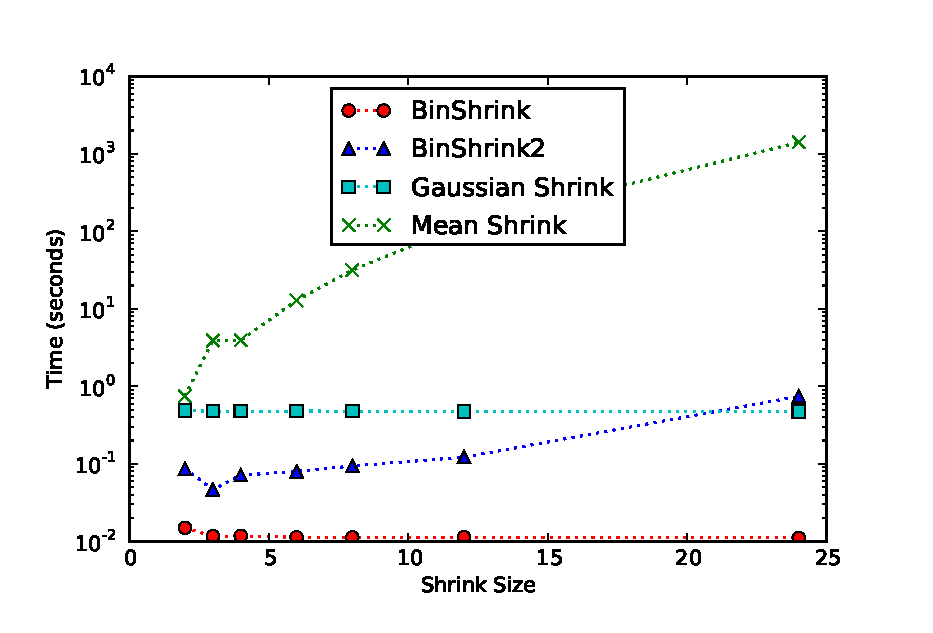
\includegraphics[width=0.8\linewidth]{images/shrink_time}
  \itkcaption{The execution time of the \textit{BinShrink} filter
    compared to the original \textit{BinShrink2} implementation and
    other shrinking approaches.}
  \label{fig:ShrinkPerformance}
\end{figure}

\begin{table}
\begin{center}
\begin{tabular}{l|*{7}{c}r}
Algorithm & \multicolumn{7}{c}{Shrink Factor} \\
  &            2 & 3 & 4 & 6 & 8 & 12 & 24 \\
\hline
BinShrink &     0.0149 & 0.0116 & 0.0118 & 0.0113 & 0.0112 & 0.0113 & 0.0110\\
BinShrink2 &    0.0862 & 0.0465 & 0.0714 & 0.0797 & 0.0940 & 0.1217 & 0.7451\\
GaussianShrink &0.4850 & 0.4779 & 0.4778 & 0.4803 & 0.4791 & 0.4752 & 0.4767\\
MeanShrink &    0.7440 & 3.9093 & 3.9264 & 12.818 & 31.602 & 121.80 & 1412.3\\
\end{tabular}
\itkcaption{The execution time in seconds of algorithms verses various
shrink factors.}
\label{tab:ShrinkPerformance}
\end{center}
\end{table}

Analyzing the difference in performance between the \textit{BinShrink}
and \textit{BinShrink2} filters is quite interesting. Both these
filters access the same number of input pixels and output pixels to
perform the same computation. The difference between them is the type of iterator
used and the order in which the images are accessed. The differences
in the iterator should account for the time difference
for a shrink factor of 2. However, the large increase in the
\textit{BinShrink2} execution times can not be explained by the
difference in the iterator operation costs. Specifically our
performance results indicate that for a shrink factor of 24 the
\textit{BinShrink} is 67X faster. We conjecture that this disparity is
due to \textit{BinShrink2}'s inefficient memory access pattern
causing decreased cache hits.

\section{Conclusion}

We have demonstrated that the \textit{BinShrink} filter is a fast
filter for multi-resolutional work. We have also shown that
by coherently accessing images in scan-line order the performance can
be improved by a factor of 10.
\textit{BinShrink} may not always be the best method for image quality as it
may result in aliasing. However, features such as wide pixel type
support and streaming make it quite practical for working with large
data sets.


\bibliographystyle{plain}
\bibliography{BinShrink}


\end{document}
